\section{Chimera Restore Session protocol}
\label{app:chimeraRestoreSession}%a030

Protocol designed to restore \chimera session, provided that this session has been saved previously in \scipion. Currently, three protocols save \chimera sessions when \chimera commands \ttt{scipionwrite} or \ttt{scipionss} are used, \scommand{chimera rigid fit}, \scommand{chimera operate} and \scommand{model from template} (Appendices \ref{app:chimeraRigidFit}, \ref{app:chimeraOperate} and \ref{app:modelFromTemplate}, respectively). Restored sessions allow inspect any element contained in a previously saved \chimera session, perform \chimera operations, and finally save electron density volumes or atomic structures.\\

 \begin{itemize}
  \item \scipion menu:\\
   \ttt{Protocols SPA -> Tools -> Calculators} (\ffigure{fig:app_protocol_chimera_3} (A))\\
  
  \item Protocol form parameters (\ffigure{fig:app_protocol_chimera_3} (B)):\\
  
    \begin{figure}[H]
     \centering 
     \captionsetup{width=.7\linewidth} 
     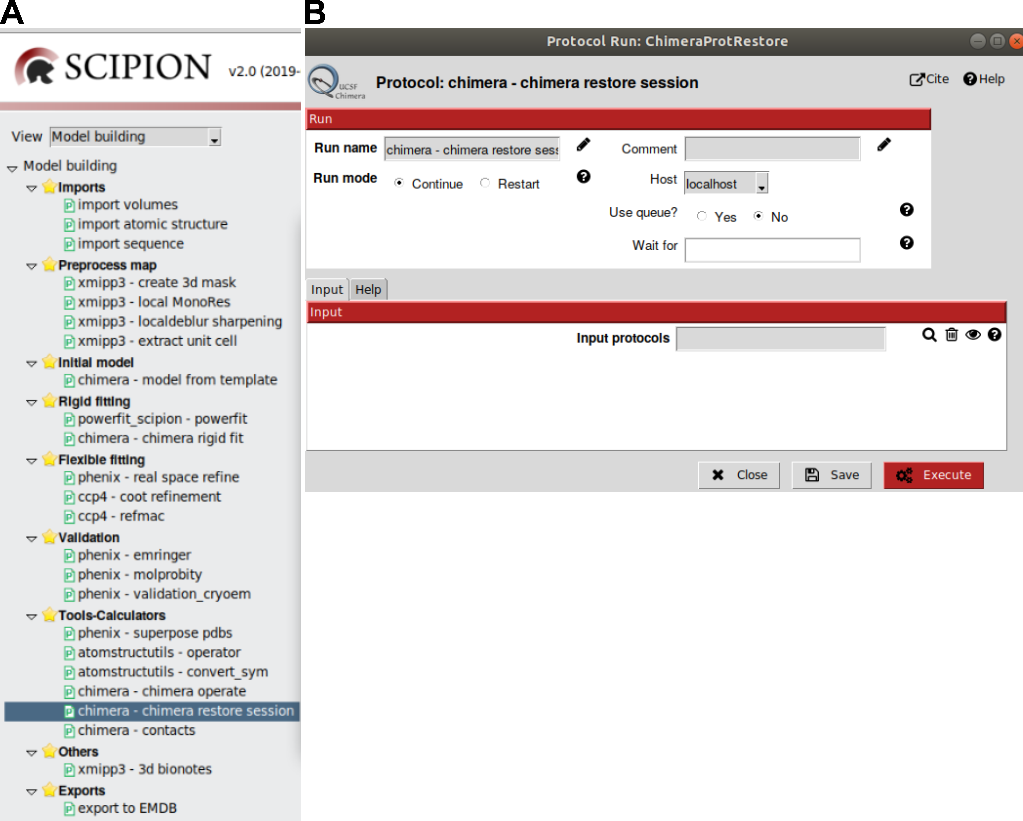
\includegraphics[width=0.90\textwidth]{Images_appendix/Fig118.pdf}
     \caption{Protocol \scommand{chimera restore session}. A: Protocol location in \scipion menu. B: Protocol form.}
     \label{fig:app_protocol_chimera_3}
    \end{figure}
    
    \begin{itemize}
     \item \ttt{Input} section\\

    \begin{itemize}
     \item \ttt{Input protocols}: Parameter that allows to select a particular protocol in which \chimera session has been saved in \scipion. As has been already mentioned above, three protocols support this possibility (\chimera \ttt{rigid fit}, \chimera \ttt{operate} and \scipion \ttt{model from template}).\\
     
    \end{itemize}
    \item \ttt{Help} section\\
    
    This section contains \chimera commands required to save $models$ according to their reference volumes, which can also be saved if required. Remark that using \ttt{scipionwrite} command, \chimera session will be saved by default, without prejudice that it may be saved with \ttt{scipionss} command. \chimera sessions can be restored again by using this same \scommand{chimera restore session} protocol.\\
    
    \end{itemize}

  \item Protocol execution:\\
  
  Adding specific protocol label is recommended in \ttt{Run name} section, at the form top. To add the label, open the protocol form, press the pencil symbol at the right side of \ttt{Run name} box, complete the label in the new opened window, press OK, and finally, close the protocol. This label will be shown in the output summary content (see below). If you want to run again this protocol, do not forget to set to \ttt{Restart} the \ttt{Run mode}.\\
  Press the \ttt{Execute} red button at the form bottom.\\
  
  \chimera graphics window will be opened after executing the protocol showing the complete list of elements that appeared in \chimera graphics window when the session was saved, coordinate axes, electron density maps, and atomic structures. Steps to follow depend on the specific operation to carry out. New volumes or structures may be generated as usual in \chimera, and they can be saved in \scipion in the common way.\\
  \begin{itemize}
   
   \item To save an atomic structure generated with this protocol:
   Write in \chimera command line:\\
   \ttt{scipionwrite model \#n}\\
   If you want to save the model regarding any electron density map, write in \chimera command line:\\
   \ttt{scipionwrite model \#n refmodel \#n saverefmodel 0/1}.\\Replace \ttt{\#n} by model numbers shown in \chimera \ttt{Model Panel}. Select \ttt{1} if you want to save the reference map or \ttt{0} if you do not want to avoid unnecessary duplicate data.\\
   \item To save a volume generated with this protocol:\\
   New volume data sets have to be saved first in a separate volume file. Otherwise those volumes will not be saved in the \chimera session since session files only record file paths to volumes. Assuming that the name chosen for the new volume generated is \ttt{volume\_name.mrc}, and \ttt{abspath} the absolute path in which you want to save the volume, write in \chimera command line:\\
   \ttt{volume \#n save abspath/volume\_name.mrc}\\
   \ttt{scipionwrite model \#n refmodel \#n saverefmodel 1}.\\Replace \ttt{\#n} by model numbers shown in \chimera \ttt{Model Panel}. Remark that you have to save an atomic structure if you want to save a volume in \scipion.\\
   \item Close \chimera graphics window.\\

 \end{itemize}
  \item Visualization of protocol results:\\
  
    After executing the protocol, press \ttt{Analyze Results} and \chimera graphics window will be opened by default. Atomic structures and volumes are referred to the origin of coordinates in \chimera. To show the relative position of atomic structure and electron density volume, the three coordinate axes are represented; X axis (red), Y axis (yellow), and Z axis (blue) (\ffigure{fig:app_protocol_volume_3}). Coordinate axes, volume, and atomic structure are model numbers \ttt{\#0}, \ttt{\#1}, and \ttt{\#2}, respectively, in \chimera \ttt{Model Panel}. If no volumes have been included, coordinate axes and each atomic structure are model numbers \ttt{\#0} and \ttt{\#1}, respectively.\\
   
  \item Summary content:\\
  
   \begin{itemize}
    \item If an atomic structure is generated:\\

    \begin{itemize}
     \item Protocol output (below \scipion framework):
      \ttt{chimera - chimera restore session -> ouputPdb\_01}; \ttt{Pdbfile (pseudoatoms=True/ False, volume=True/ False)}.\\Pseudoatoms is set to \ttt{True} when the structure is made of pseudoatoms instead of atoms. Volume is set to \ttt{True} when an electron density map is associated to the atomic structure.\\
     \item \ttt{SUMMARY} box:\\Produced files:\\chimeraOut0001.pdb\\we have some result\\
    \end{itemize}
    \item If a volume is generated:\\
    
    \begin{itemize}
     \item Protocol output (below \scipion framework):
      \ttt{chimera - chimera restore session -> ouput3Dmap}; \ttt{Volume (x, y, and z dimensions, sampling rate)}.\\
      \ttt{chimera - chimera restore session -> ouputPdb\_01}; \ttt{Pdbfile (pseudoatoms=True/ False, volume=True/ False)}.\\Pseudoatoms is set to \ttt{True} when the structure is made of pseudoatoms instead of atoms. Volume is set to \ttt{True} when an electron density map is associated to the atomic structure.\\
     \item \ttt{SUMMARY} box:\\Produced files:\\chimeraOut0001.pdb\\chimeraOut0001.mrc\\we have some result\\
    \end{itemize}
    
   \end{itemize}
  
 \end{itemize}
